\newpage
\chapter{Приближени пресмятания - подходи, методи, алгоритми}
\label{chapter10}
\thispagestyle{empty}

В изчислителната математика се открояват две основни направления – точните числени пресмятания и приближените числени пресмятания\index{приближени пресмятания}. Точни числени пресмятания\index{точни числени методи} се извършват в ситуации в които обемът на задачата позволява изчисленията да се осъществят в приемлив интервал от време. В реалната практика често поставяните задачи значително нарастват като обем и тяхното пресмятане с точени числени методи става неприемливо по отношение на нужното време за пресмятане. В такива ситуации се прибягва до множеството разработени методи за приближени пресмятания\index{приближени числени методи}. По отношение на програмния продукт R, ще бъдат разгледани някои от най-популярните методи за приближени числени пресмятания, а именно Монте-Карло симулации, генетични алгоритми и изкуствени невронни мрежи.

\section{Монте-Карло методи}

В средата на XX век, във връзка с разработването на първите ядрени оръжия, са разработени група методи за приближени пресмятания, които залагат на способ за генериране на голямо количество случайни числа и последващата им статистическа обработка. Монте-Карло методите\index{Монте-Карло методи} намират най-голямо приложение в оптимизационни задачи, числено интегриране и генериране на семпли за специфични вероятностни разпределения. Монте-Карло методите могат да се използват за решаването на всяка задача, която има представяне в термините на вероятности и статистика. 

Има вариации в реализацията на Монте-Карло методите, но те в общия случай следват няколко добре дефинирани стъпки:

1. Определяне на област от допустими стойности;

2. Генериране на извадка от случайни числа в предварително дефинираната област;

3. Извършване на точни пресмятания с така генерираните случайни числа;

4. Обобщаване на резултатите от извършените пресмятания.

\begin{figure}[h!]
  \centering
  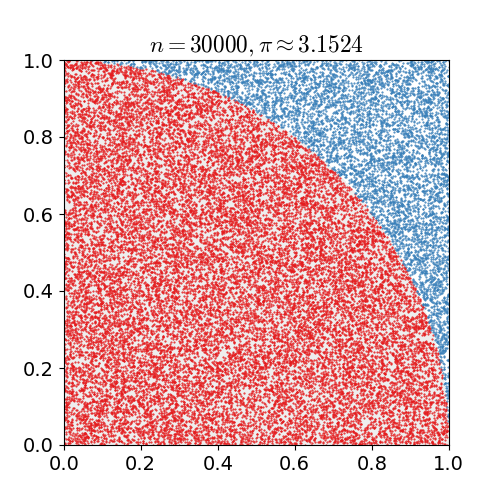
\includegraphics[width=0.8\linewidth]{pic0060}
  \caption{Пресмятане на числото $\pi$ с Монте-Карло метод}
\label{figure0060}
\end{figure}
\FloatBarrier

Един от най-популярните примери за Монте-Карло пресмятане е приближеното изчисление на числото $\pi$ (Фиг. \ref{figure0060}). За тази цел една четвърт от окръжност се представя с обгръщащия я квадрат. Съотношението между площите на квадрата и на четвъртината окръжност е $\pi/4$. За да се апроксимира стойността на числото $\pi$ с Монте-Карло метод се изпълняват следните стъпки:

1. Изчертаване на квадрат и четвъртина окръжност вписана в него;

2. Генериране на случайни равномерно разпределени числа, като координати (x,y двойки) в описаната допустима област;

3. Изброяване на точките с координати x,y които са на разстояние 1 от центъра на четвърт окръжността; 

4. Съотношението между точките в четвърт окръжността и общия брой точки е $\pi/4$, което умножено по 4 дава приближена стойност за числото $\pi$. 

При тази процедура за приближено пресмятане е важно да се вземат под внимание два много важни фактора:

1. Ако генерираните случайни числа не са равномерно разпределени, това ще доведе до невярна апроксимация за търсената стойност;

2. Генерирането на малък брой координати за точки в дефиниционната област води до ниско надеждна стойност за апроксимация, което означава, че колкото по-голям обем е извадката от случайни числа, толкова по-надеждни резултати за апроксимация.

\begin{lstlisting}[caption=Монте-Карло пресмятане, label=listing0175]
library( MonteCarlo )

mode <- function(x) {
	values <- unique(x)
	return( values[which.max(tabulate(match(x, values)))] )
}

experiment <- function(n, d){
	x <- sample(6,n,TRUE)

	for(i in 2:d) {
		x <- x + sample(6,n,TRUE)
	}

	return( list("mean"=mean(x), "median"=median(x), "mode"=mode(x)) )
}

result <- MonteCarlo(func=experiment, nrep=1000, param_list=list("n"=c(10, 50, 100, 150, 200),"d"=c(1,2,6)))

summary( result );

MakeTable(output=result, rows=c("d"), cols=c("n","list"), digits=2, include_meta=FALSE)
\end{lstlisting}

Към програмния продукт R е създаден отделен пакет (автор Christian Hendrik Leschinski) за извършване на Монте-Карло пресмятания, наречен „MonteCarlo“ (Листинг \ref{listing0175}). 

За демонстрация на възможностите, които R дава при Монте-Карло симулации е представено сравнение между средната, медианата и модата за вероятностно разпределение на сумата от $n$ зара. Тъй като R не предлага функция за пресмятане на мода е необходимо тази функция да бъде предварително дефинирана (Листинг \ref{listing0175}).

В пакета $MonteCarlo$\index{Монте-Карло методи} основно се използват две функции - $MonteCarlo$ и $MakeTable$. Функцията $MonteCarlo$ има за основна задача генерирането на множеството експерименти в процеса на симулацията. Най-важният параметър за тази функция е функционален обект, който описва единичен експеримент. В програмния език R функционалните обекти по своята същност представляват потребителски дефинирани функции. В предложения пример функционалният обект се нарича $experiment$, а функцията която представлява получава два входни параметъра $n$ и $d$. Потребителят на пакета $MonteCarlo$ сам може да избира какъв брой параметри да има функцията за единичен експеримент. В настоящия пример $n$ определя броят случайни числа, които да бъдат генерирани (размер на случайната извадка), а $d$ определя колко зара ще участват във формирането на крайния резултат. При предишни примери бе показано, че вероятностното разпределение на един зар е равномерно, на два зара триъгълно, а при достатъчно много зарове разпределението клони към нормалното. В този пример се разглеждат разликите между средната, медианата и модата за 1, 2 и 6 зара.

Към функцията за единичен експеримент има следните изисквания: 1. Аргументите а бъдат скаларни стойности; 2. Върнатата стойност от функцията да бъде списък с именувани или неименувани скаларни стойности. Потребителската функция за единичен експеримент се изпълнява в текущото работно пространство и поради тази причина всички нужни библиотеки, променливи с данни и помощни функции трябва да са заредени предварително. 

Вторият важен аргумент на функцията $MonteCarlo$ е $param_list$ и трябва да изпълнява следните изисквания: 1. Трябва да е списъчна структура; 2. Елементите на списъка трябва да са именувани и имената да съответстват на имената използвани за параметри в потребителската функция за единичен експеримент; 3. Всеки елемент в списъка е вектор със скаларни стойности; 4. Списъкът съдържа точно толкова на брой елементи, колкото са параметрите на потребителската функция за единичен експеримент. 

Последният задължителен аргумент на функцията $MonteCarlo$ е $nrep$ и той определя колко пъти ще бъде изпълнен Монте-Карло експериментът. В представения пример (Листинг \ref{listing0175}) се изпълняват хиляда повторения за три възможни комбинации от зарове, при пет различни броя за хвърлянето на тези зарове, а именно 10, 50, 100, 150 и 200. 

\begin{table}[h]
\centering
\resizebox{ 1 \textwidth}{!}{%
\begin{tabular}{ rrrrrrrrrrrrrrrrrrr }
\hline\hline\\\\
 list && \multicolumn{ 5 }{c}{ mean } &  & \multicolumn{ 5 }{c}{ median } &  & \multicolumn{ 5 }{c}{ mode } \\ 
d/n &  & 10 & 50 & 100 & 150 & 200 &  & 10 & 50 & 100 & 150 & 200 &  & 10 & 50 & 100 & 150 & 200 \\ 
 &  &  &  &  &  &  &  &  &  &  &  &  &  &  &  &  &  &  \\ 
1 &  & 10.50 & 10.48 & 10.49 & 10.50 & 10.50 &  & 10.52 & 10.50 & 10.48 & 10.50 & 10.52 &  & 10.48 & 10.50 & 10.42 & 10.49 & 10.53 \\ 
2 &  &  7.01 &  7.00 &  7.00 &  7.01 &  6.99 &  &  7.02 &  7.01 &  7.00 &  7.00 &  7.00 &  &  7.03 &  7.04 &  6.98 &  6.98 &  6.99 \\ 
6 &  & 20.94 & 21.03 & 21.00 & 21.01 & 21.00 &  & 20.90 & 21.01 & 20.99 & 21.00 & 21.00 &  & 20.86 & 20.98 & 21.04 & 21.00 & 20.97 \\ 
\\
\\
\hline\hline
\end{tabular}%
}
\caption{Сравнение на средна, медиана и мода за експеримент със зарове}
\label{table0005}
\end{table}

За визуализация на получените резултати от функцията $MonteCarlo$ се използва функцията $MakeTable$. На функцията $MakeTable$ се подава резултата от симулацията и тя генерира таблица с резултати в $LaTeX$ формат (Таб. \ref{table0005}).

Функцията $MakeTable$ дава множество възможности, но само три от аргументите й са задължителни. На аргумента $output$ се присвоява резултата от изпълнението на функцията $MonteCarlo$. Вторият и третият аргумент са $rows$ и $cols$, като те определят по какъв начин ще се организират табличните данни. В представения пример (Листинг \ref{listing0175}) по редове са организирани броя зарове участващи в единичен експеримент, а по колони са организирани броят хвърляния на заровете, групирани по вида статистика (средна, медиана или мода). 

Макар и незадължителен параметърът $digits$ е определен на 2, което дава по-добра прегледност на табличната визуализация. Също незадължителен параметърът $include_meta$ е установен на „лъжа“ с цел да не се генерират коментари с обобщаваща информация за извършената симулация. 

\section{Генетични алгоритми}

Генетичните алгоритми\index{генетични алторитми} са евристика за глобална оптимизация, която е вдъхновена от идеите за естествената природна еволюция. Генетичните алгоритми са спадат към по-голям клас оптимизационни евристики наречени „еволюционни алгоритми“\index{еволюционни алгоритми}. Основното си приложение генетичните алгоритми намират в оптимизационни задачи в големи пространства. По-своята същност генетичните алгоритми са вероятностни и генерират субоптимални решения, като относително рядко достигат до глобалния опитимум. Изчисленията при генетичните алгоритми са организирани в три основни операции (рекомбинация) – селекция, кръстосване и мутация. Пресмятанията най-често започват от група случайно генерирани решения, които съставят първоначалната популация. Целта е в процеса на еволюция решенията системно да се подобряват. Популацията условно се разделя на старо и ново поколение. В новото поколение влизат решенията генерирани след рекомбинацията. За всяко решение в популацията се определя стойност на жизнеспособност. В общия случай стойността на жизнеспособност е резултата от пресмятането на функцията, която подлежи на оптимизация. Най-жизнеспособните решения биват подбрани да участват в създаването на новото поколение. Създаването на нови поколения е итеративен процес и най-често той приключва след изтичането на определен брой поколения или достигане на задоволително ниво за оптималност на предложеното решение. 

Генетичните алгоритми представят информацията под формата на група от решения организирани в популация. Всяко решение представлява вектор от стойности в пространството на решенията. Кодирането на задачата в термините на генетичните алгоритми е строго специфично за всяка задача. При целочислени задачи стойностите във вектора са цели числа. При пресмятане на непрекъснати задачи стойностите на вектора са реални числа. При някои комбинаторни задачи кодирането е под формата на пермутации. В повечето случаи дължината на вектора е фиксирана, но това не е задължително условие. Примерно при кодиране на серия от инструкции за конкретна машина, дължината на серията може да варира. Най-често началната популация се генерира на случаен принцип, но това не е задължително, особено ако се налага оптимизацията да продължи от вече постигнати резултати. Съществен е въпросът за размера на популацията и в практиката се е наложило този размер да се определя експериментално. При селекцията е от значение най-жизнеспособните решения да имат най-голям шанс за възпроизвеждане, но в същото време е важно и по-слабите решения да има шанс за участие в следващото поколение. 

Оценката на жизнеността най-често се постига, чрез подаване на решението към целевата функция. Целевата функция е строго специфична за всяка различна задача, която се решава. Желателно е целевата функция да връща единствена стойност. Ако при оптимизационната задача има повече критерии за оптимизиране, то многокритериалната задача трябва да се сведе до еднокритериална. След избора на два (или повече) родители, операцията по кръстосване разменя части от векторите. С помощта на кръстосването се изследват обширни региони от пространството на решенията. При мутацията на случаен принцип в новото поколение се избират отделни елементи от вектора и те се модифицират. Мутацията спомага за изследването на близки околности във вече генерираните точки в пространството на решенията. 

Използването на генетични алгоритми става неефективно в ситуации в които целевата функция изисква неприемливо дълго време за пресмятане. Тъй като генетичните алгоритми ползват генерирането на голямо количество междинни решения, множеството пресмятания на целевата функция може да направи цялата оптимизация неприемливо бавна. Важно е също да се знае, че генетичните алгоритми не гарантират намирането на глобалния оптимум, най-вече когато този оптимум не е предварително известен. Генетичните алгоритми не са ефективни при задачи където целевата функция води само до две състояния „добро“ или „лошо“. За да бъде ефективен процесът по оптимизацията решенията в популацията трябва да подлежат на подреждане, спрямо тяхната жизнеспособност. 

\begin{table}[h!]
\centering
\begin{tabular}{|l|r|r|} 
  \rowcolor{lightgray}
  \hline
  Предмет & Ценност & Тегло \\ [0.1ex] 
  \hline\hline
  cake & 10 & 1 \\
  \hline
  ice cream & 15 & 10 \\
  \hline
  orange juice & 10 & 5 \\
  \hline
  strawberries & 30 & 7 \\
  \hline
  grape & 30 & 1 \\
  \hline
  candies & 20 & 5 \\
  \hline
  chocolate & 2 & 1 \\
  \hline
\end{tabular}
\caption{Предмети с определена ценност и тегло}
\label{table0006}
\end{table}

Възможностите за оптимизация с генетични алгоритми добре може да се илюстрира с една от най-популярните комбинаторни задачи, която се нарича „задача на раницата“. Всяка раница има ограничена вместимост и максимално тегло, което човекът може да носи. В същото време има множество предмети, които биха били полезни, ако са налични при едно пътуване. Всеки предмет има своя специфична ценност, която е важна за притежателя му, но също така има и специфично тегло. Целта на оптимизацията е да се вземат тези предмети на които сумарното тегло не надвишава лимита, но и носят максимална сумарна ценност. Тази задача е от областта на целочислената оптимизация и дали един предмет попада в групата на взетите може да се отбележи с единица, а ако не попада в тази група с нула. Макар и да изглежда проста задачата за раницата е много трудно решима, особено когато става въпрос за много на брой предмети и силно ограничено сумарно тегло, какъвто е случаят с изстрелването на летателни апарати в космоса. В представения пример са изброени група храни и напитки, които човек би избрал за разходка в планината (Таб. \ref{table0006}). 

\begin{lstlisting}[caption=Оптимизация на задачата за раницата с генетични алгоритми, label=listing0176]
library(genalg)

data <- data.frame(item = c("cake", "ice cream", "orange juice", "strawberries", "grape", "candies", "chocolate"), points = c(10, 15, 10, 30, 30, 20, 2), weight = c(1, 10, 5, 7, 1, 5, 1))

limit <- 20

solution <- c(1, 0, 0, 1, 1, 0, 0)

data[solution==1, ]
#           item         points weight
# 1         cake             10      1
# 4 strawberries             30      7
# 5        grape             30      1

cat(solution %*% data$points)
# 70

# Fitness function calculation.
fitness <- function(x) {
	points <- x %*% data$points

	weight <- x %*% data$weight

	if (weight > limit) {
		return( 0 )
	} else {
		return( -points )
	}
}

iterations <- 75

model <- rbga.bin(size=7, popSize=37, iters=iterations, mutationChance=0.01, elitism=TRUE, evalFunc=fitness)

cat( summary(model) )
# GA Settings
#   Type                  = binary chromosome
#   Population size       = 37
#   Number of Generations = 75
#   Elitism               = TRUE
#   Mutation Chance       = 0.01
# 
# Search Domain
#   Var 1 = [,]
#   Var 0 = [,]
# 
# GA Results
#   Best Solution : 1 0 1 1 1 1 1 

# Print the best found solution.
best <- c(1, 0, 1, 1, 1, 1, 1)
data[best == 1, ]
#           item         points weight
# 1         cake             10      1
# 3 orange juice             10      5
# 4 strawberries             30      7
# 5        grape             30      1
# 6      candies             20      5
# 7    chocolate              2      1

# Calculate survival points.
cat(paste(best %*% data$points, "/", sum(data$points)))
# 102 / 117
\end{lstlisting}

За използването на генетични алгоритми в R една от възможностите е пакетът $genalg$ (Листинг \ref{listing0176}). Основната функция в този пакет за работа с бинарни вектори на решенията е $rbga.bin$ и като резултат от извикването й се получава обект с модела на извършената оптимизация. Параметърът $size$ определя каква е размерността на пространството. В разглеждания пример са налични 7 обекта и поради тази причина векторът описващ едно решение има 7 компонента. Параметърът $popSize$ определя какъв да бъде размерът на популацията\index{размер на популация}. Тъй като няма разработена теория за определяне на този размер, той се определя експериментално и най-подходящата стойност варира от задача до задача. Препоръчително е да се изпробват различни стойности за да се провери при коя оптимизацията протича най-ефективно. Параметърът $iters$ определя от колко итерации да се състои процесът по оптимизация. При задачи в пространства с голям брой измерения този параметър може да се наложи да има голяма стойност. В представения пример бройката от 75 итерации се оказва напълно достатъчна. Параметърът $mutationChance$ определя колко често, на вероятностен принцип, да се случва мутацията на отделни елементи във векторите на решенията. Емпирично правило е стойността на този параметър да бъде относително малко число. В много случаи на оптимизация с генетични алгоритми по-добри резултати се постигат, когато се използва правилото за елита\index{елит}, което се контролира с булев аргумент $elitism$. За да работи ефективно оптимизацията с генетични алгоритми е нужно да се изпрати и аргумент $evalFunc$ към обект от тип функция, който да служи за изчисляване на жизнеността за всеки вектор на решение. 

В представения пример функцията за жизненост е наречена $fitness$ и като входен аргумент получава само един вектор, представляващ вектор на единично решение. При задачата за раницата сумарното тегло на избраните за натоварване предмети определя и до колко един вектор на решение е жизнеспособен. При надхвърляне на лимита се използва малък трик, стойността на жизнеността да бъде направена отрицателна (Листинг \ref{listing0176}). По този начин решения, които са с голямо надхвърляне на позволения лимит биха били оценени с най-слаба стойност за жизненост. 

За удобство, описанието на данните е организирано в $data.frame$ структура, която съдържа вектор с названията на обектите, вектор с ценността на всеки предмет и вектор с теглото на всеки предмет (Листинг \ref{listing0176}). Обекта с данните, лимита за максимално тегло и броят итерации са представени като обекти в общото пространство на текущата R сесия, така че функцията за оценка на жизнеността да има директен достъп до тази информация. След извършване на оптимизацията с помощта на функцията $summary$ може да се визуализира най-доброто открито решение. 

В представения пример оптималното решение предложено от генетичния алгоритъм изключва само един предмет $ice creea$, като достига 102 точки на полезност от максималните 117 точки на полезност. Ако експериментът бъде повторен с лимит на раницата от 15 се получава решение в което не участват $ice cream$ и $orange juice$. При този лимит постигнатата оптимална стойност е 92 от 117. 

\begin{lstlisting}[caption=Анимирана визуализация на процеса по търсене на оптимално решение, label=listing0177]
library(ggplot2)
library(animation)

setwd("~/Desktop")

animate <- function(x) {
	for (i in seq(1, iterations)) {
		current <- data.frame(Generation = c(seq(1, i), seq(1, i)), Variable = c(rep("mean", i), rep("best", i)), Survivalpoints = c(-model$mean[1:i], -model$best[1:i]))

		graphics <- ggplot(current, aes(x = Generation, y = Survivalpoints, group = Variable, colour = Variable)) + geom_line() + scale_x_continuous(limits = c(0,  iterations)) + scale_y_continuous(limits = c(0, 110)) + geom_hline(yintercept = 0, y = max(current$Survivalpoints), lty = 2) + annotate("text", x = 1, y = max(current$Survivalpoints) + 2, hjust = 0, size = 3, color = "black", label = paste("Best Found Solution:", max(current$Survivalpoints))) + scale_colour_brewer(palette = "Set1") + labs(title = "Evolution Knapsack Optimization Model")

		print( graphics )
    }
}

saveGIF(animate(), interval=0.1, outdir=getwd())
\end{lstlisting}

При извършването на оптимизация с приближени числени методи винаги от голямо значение е да се наблюдава сходимостта на процеса\index{сходимост на процес}. Благодарение на възможностите за създаване на анимирани GIF файлове, която пакетът $animation$, сходимостта на процеса по оптимизация на предложената задача за раницата може да бъде наблюдаван (Листинг \ref{listing0177}).

\begin{figure}[h!]
  \centering
  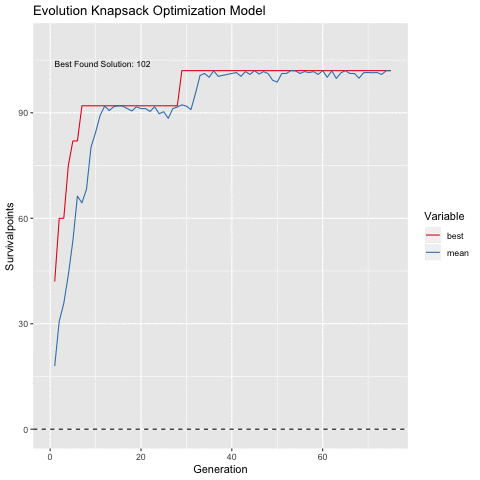
\includegraphics[width=0.8\linewidth]{pic0061}
  \caption{Сходимост на процеса по оптимизация}
\label{figure0061}
\end{figure}
\FloatBarrier

По своята същност кадровата анимация представлява последователност от отделни изображения, генерирани с помощта на функциите в пакета $ggplot2$. За всяка итерация от оптимизацията се генерира отделно статично растерно изображение (Листинг \ref{listing0177}). В генерираната анимация\index{анимация} се проследява текущо намерената оптимална стойност, най-доброто открито решение и средната стойност на решенията в популацията (Фиг. \ref{figure0061}). Тъй като генетичните алгоритми имат стохастична\index{стохастичен алгоритъм} природа, то всяко стартиране на кода от примера ще води до различно решение, но близко до оптималното. 

\section{Изкуствени неверонни мрежи}

Изкуствените невронни мрежи\index{изкуствени невронни мрежи} започват своето развитие в средата на XX век, като пред 80 години добиват нова популярност, а към настоящия момент са един от най-обещаващите методи за приближени пресмятания в областта на изкуствения интелект\index{изкуствен интелект}. Работата по изкуствените неверонни мрежи започва с идеята да се направи математически модел на естествените биологични нервни системи. Разбира се, толкова амбициозна задача се оказва не толкова лесно приложима и в резултат на тези усилия се появява клон в числените пресмятания наречен „изкуствени невронни мрежи“, които за жалост са много далеч от реален модел на биологична нервна система. 

Най-голямото предимство на изкуствените невронни мрежи е тяхната възможност да се обучават с помощта на примери. В общия случай изкуствените невронни мрежи са съставени от голям брой малки, но взаимно свързани елементи наречени неврони. Обработката на информацията е нелинейна и в силно паралелна топология на мрежата. Изкуствените невронни мрежи попадат в категорията на само-адаптиращите се системи. Това означава, че мрежата може да промени своето поведение, спрямо примерите с които бива обучавана в течение не времето. 

Най-основното си приложение изкуствените невронни мрежи намират при решаването на задачи, които се решават с лекота от хората, но са трудни за решаване с класическите изчислителни машини. Пример за такива задачи са разпознаването на лица, разпознаването на пръстови отпечатъци, разпознаването на печатен или ръкописен текст, прогнозирането на времеви редове и много други. Общото название на тази група задачи е „разпознаване на образи“\index{разпознаване на образи}. Под „образ“ се разбира по-широкото понятие, а не тясно свързаното с графично изображение. 

Най-широко разпространеният вид изкуствена невронна мрежа е трислойният перцептрон\index{многослоен перцептрон}. По своята същност този вид невронна мрежа представлява насочен тегловен граф\index{насочен тегловен граф} организиран а слоеве. Теоретично е доказано, че трислойна мрежа може да научи всяка функция представена с примери за вход изход. При съвременните реализации на многослойни перцептрони се използват значително по-голям брой слоеве, но принципа на работа остава един и същ. При многослойните перцептрони е характерно всеки слой да бъде пълно свързан с предхождащия и със следващия (Фиг. \ref{figure0065}). Към всеки слой има допълнителен неврон, който не получава входни сигнали и служи за отместване (bias). Този неврон емитира единичен сигнал към следващия слой. Входният слой получава информация от външната среда за мрежата, тоест не е свързан с предходен слой. Изходният слой подава резултата от изчислението на мрежата към външната среда, тоест няма свързване към следващ слой. Мрежата съхранява научената информация в своите тегла и процесът на обучение е пряко свързан с такава модификация на теглата в графа, че мрежата да постига оптимални резултати в работен режим. 

Най-големият недостатък на изкуствените невронни мрежи е нуждата от много време през фазата на обучението. Разработени са множество точни числени методи за модифициране на теглата в мрежата, като най-популярният е обратно разпространение на грешката\index{обратно разпространение на грешката}. Този метод е градиентен точен числен метод и дава едни от най-добрите резултати при обучението на многослойни перцептрони. Разработени са също и приближени числени методи за модификация на теглата в мрежата, като един от най-популярните е еволюция на разликите\index{еволюция на разликите}. Еволюция на разликите е модификация на генетичен алгоритъм в частта му са операцията по мутация. Най-голямото предизвикателство в съвременното развитие на изкуствените невронни мрежи е намирането на възможно по ефективни топологии на мрежата и намирането на възможно по-бързи алгоритми за обучение на мрежата. 

\begin{figure}[h!]
  \centering
  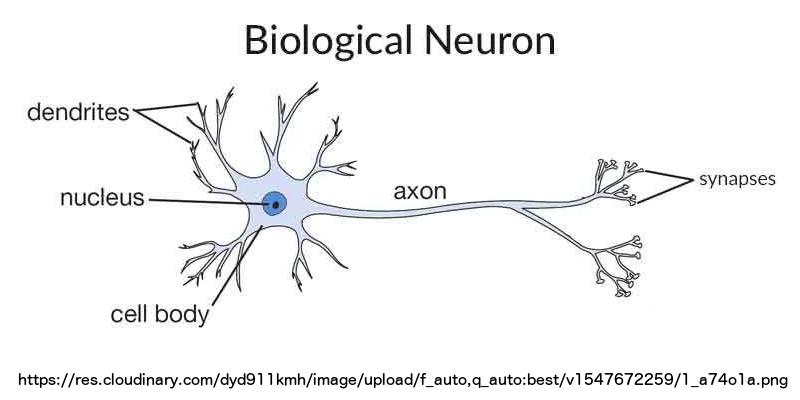
\includegraphics[width=1.0\linewidth]{pic0062}
  \caption{Схема на биологична нервна клетка}
\label{figure0062}
\end{figure}
\FloatBarrier

В биологичните неврони клетката има тяло, свързано с дендрити за входни сигнали, ядро, аксон предаващ сигнала към синапсите (Фиг. \ref{figure0062}). По аналогия с биологичния неврон, изкуственият неврон (Фиг. \ref{figure0063}) има входни връзки с тегла (дендрити), сумираща функция (ядро на неврона), функция за активация (аксон) и изходен сигнал (синапси).

\begin{figure}[h!]
  \centering
  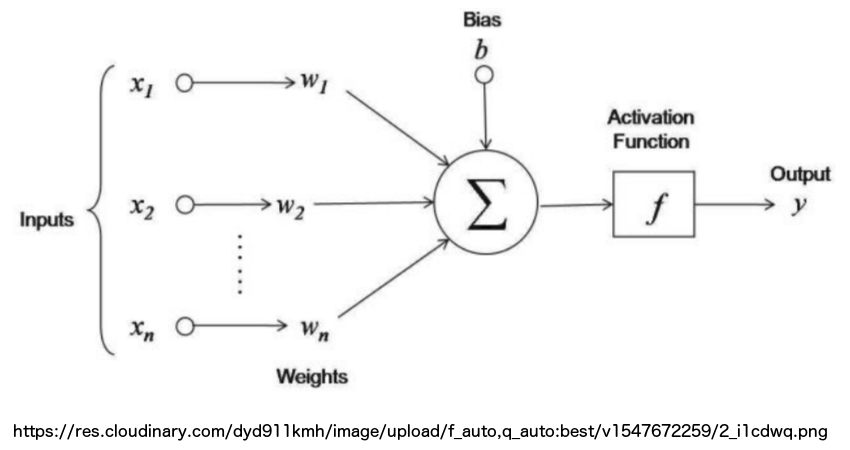
\includegraphics[width=1.0\linewidth]{pic0063}
  \caption{Схема на изкуствен неврон}
\label{figure0063}
\end{figure}
\FloatBarrier

Като трансферна функция най-често се използва линейна зависимост. Това означава, че стойността в ядрото на изкуствения неврон е сума от умножението на входните сигнали с прилежащите им тегла (Формула \ref{equation0016}). 

\begin{equation}
y_i = \sum{(w_{ij}*y_j)} + b
\label{equation0016}
\end{equation}
\listofequations{Трансферна функция в изкуствен неврон}

Тъй като няма ограничение за стойностите на теглата, то е възможно теглата да бъдат големи отрицателни числа или големи положителни числа. Сигналите на изхода на невроните е обичайно да бъдат нормирани или в диапазона от 0.0 до 1.0 или в диапазона от 1.0 до +1.0. Също така, броя входящи връзки към един неврон може да варират. При тези условия, когато се прилага линейна трансформация на сигналите (Формула \ref{equation0016}) резултата от пресмятането става несравним между различните неврони и не може разумно да се определи кой неврон какво влияние трябва да оказва към следващия слой. Това налага резултата от трансферната функция\index{трансферна функция} да бъде подложен на нормализация, чрез прилагането на функция за активация (Фиг. \ref{figure0063}). Най-често прилаганите функции за активация\index{активационна функция} имат асимптотична сходимост в минус безкрайност и в плюс безкрайност. Това са плавно нарастващи диференцируеми функции (Фиг. \ref{figure0064}). Предимството на хиперболичния тангенс пред сигмоидната функция е, че той има симетрия спрямо абсцисната ос.

\begin{figure}[h!]
  \centering
  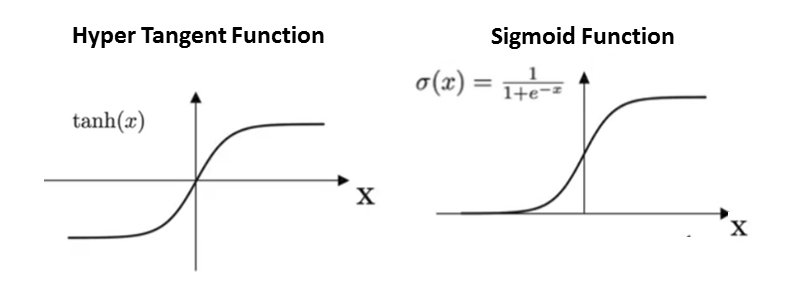
\includegraphics[width=1.0\linewidth]{pic0064}
  \caption{Функции за активация на изкуствен неврон}
\label{figure0064}
\end{figure}
\FloatBarrier

За илюстрация на възможностите, които една трислойна неврона мрежа има ще бъде използвано множество от данни за успешно започване на работа при професията „програмист“ (Таб. \ref{table0007}). Отделните кандидати са оценени по скала от 100 точки за два критерия – технически умения и социални умения. Успешно започналите работа кандидати са обозначени с „Да“, а неуспешните кандидати с „Не“. Тази организация на данните показва нуждата от въвеждане на числена информация на входа на мрежата и определянето на резултат в два класа (Да/Не).

\begin{table}[h!]
\centering
\begin{tabular}{|l|r|r|} 
	\rowcolor{lightgray}
	\hline
	Technical Skills (TS) & Soft Skills (SS) & Successful Employment (SE) \\
	\hline\hline
	30 & 80 & Yes \\
	\hline
	10 & 20 & No \\
	\hline
	20 & 90 & Yes \\
	\hline
	30 & 40 & No \\
	\hline
	80 & 50 & Yes \\
	\hline
\end{tabular}
\caption{Тренировъчно множество данни}
\label{table0007}
\end{table}

При два числени входни параметъра и един параметър за прогнозиране е съвсем естествено топологията на изкуствената невронна мрежа да бъде с два входни неврона и един изходен неврон. Остава единствено да се вземе решение за размера на скрития слой. Тъй като не е създадена теория за избор на размера на скрития слой, този размер най-често в практиката се определя експериментално. В предложения случай се използват четири неврона в скрития слой, но приемливи резултати биха се получили и с три неврона. Съкратеният записа за такава топология на изкуствена невронна мрежа е 2-4-1 и отразява бройката на невроните във всеки от слоевете. 

\begin{lstlisting}[caption=Класифициране с изкуствена невронна мержа, label=listing0178]
library(neuralnet)

training <- data.frame(TS=c(30,10,20,30,80), SS=c(80,20,90,40,50), SE=c(1,0,1,0,1))

network <- neuralnet(SE~TS+SS, data=training, hidden=4, act.fct="tanh", linear.output=FALSE)

plot(network)

testing <- data.frame(TS=c(85,30,20), SS=c(10,20,75))

prediction <- compute(network, testing)

prediction$net.result
#           [,1]
# [1,] 0.3322677
# [2,] 0.3322677
# [3,] 0.9924267

ifelse(prediction$net.result>0.5, TRUE, FALSE)
#       [,1]
# [1,] FALSE
# [2,] FALSE
# [3,]  TRUE
\end{lstlisting}

За работа с невронни мрежи в R е създаден програмният пакет $neuralnet$. За нуждите на експеримента данните се подготвят в две множества – тренировъчно и тестово (Листинг \ref{listing0178}). След което следва изграждането на модела с помощта на функцията $neuralnet$. Като първи аргумент функцията получава обект от тип формула $SE\char`\~TS+SS$, който показва кои променливи ще са на входа и кои на изхода. Параметърът $hidden$ определя размера на скрития слой. Параметърът $act.fct$ задава каква функция на активация да имат невроните. Изходът да не бъде линейно интерпретиран се задава в параметъра $linear.output$.

\begin{figure}[h!]
  \centering
  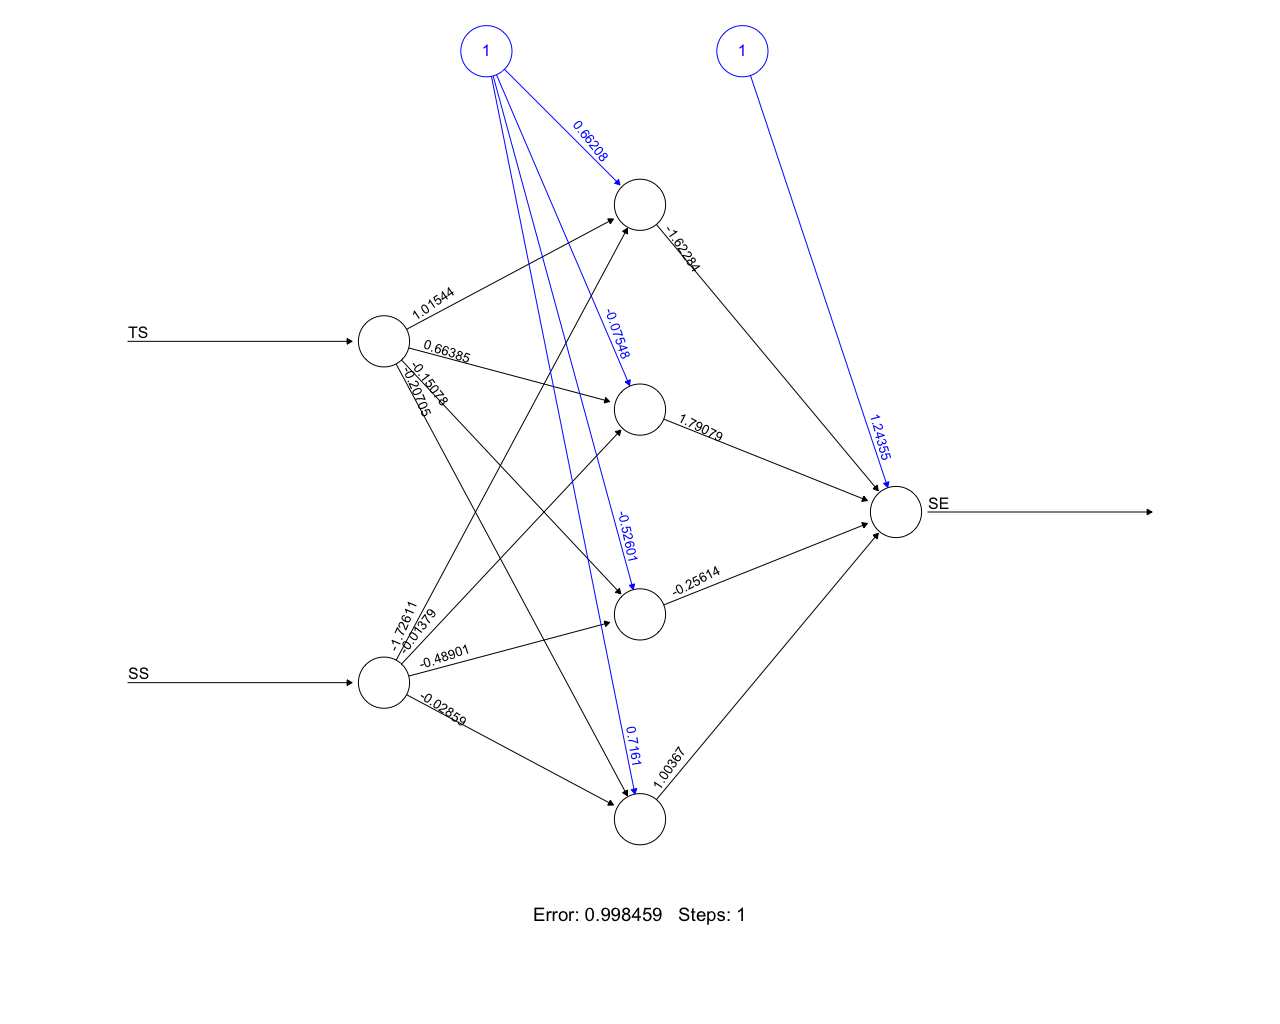
\includegraphics[width=1.0\linewidth]{pic0065}
  \caption{Трислойна изкуствена невронна мрежа}
\label{figure0065}
\end{figure}
\FloatBarrier

Изчертаването на изкуствената невронна мрежа се постига с функцията $plot$, на която се подава като аргумент самата мрежа (Фиг. \ref{figure0065}). С помощта на функцията $compute$ тестовото множество (Таб. \ref{table0008}) се подава на изкуствената невронна мрежа и се пресмятат шансовете\index{прогнозиране} за наемане на кандидатите, които не са участвали в множеството за обучение на мрежата.

\begin{table}[h!]
\centering
\begin{tabular}{|l|r|r|} 
	\rowcolor{lightgray}
	\hline
	Technical Skills & Soft Skills & Employment Forecast \\
	\hline\hline
	85 & 10 & 0.3322677 \\
	\hline
	30 & 20 & 0.3322677 \\
	\hline
	20 & 75 & 0.9924267 \\
	\hline
\end{tabular}
\caption{Тестово множество данни}
\label{table0008}
\end{table}

За ад се даде еднозначен отговор за шансовете на един кандидат дали ще бъде нает е удачно полученият резултат да се бинаризира (Листинг \ref{listing0178}).

\section*{Заключение}

В реалната практика, когато точните числени методи не успяват да дадат желаният резултат в приемливо време за пресмятане, изключително полезни могат да бъдат алгоритмите за приближени пресмятания. За симулации това са Монте-Карло методите, за оптимизация това са генетичните алгоритми, а за класификацията това са изкуствените невронни мрежи. Разбира се, съществуват множество други подходи, методи и алгоритми за приближени числени пресмятания, но представените в настоящото изложение са едни от най-използваните в практиката.

